% !TeX root = ../main.tex

\subsection{Efficiency Evaluation (RQ2)}

% Table \ref{tab:performance} presents the performance results of \tool. We denote $\tool_{P}$, $\tool_{N}$, and $\tool_{M}$ as the three models trained by PyPI packages, NPM packages, and mixed packages, respectively. 

We measure the time overhead of \tool for training and prediction, including all components described in Section~\ref{approach}. \tool is trained on a machine with an Intel Xeon(R) Silver 4314 CPU at 2.40GHz, 128G of RAM and an NVIDIA GeForce RTX 3090. The same machine is employed~for predictions. \tosemrevision{Table \ref{tab:performance} presents the efficiency results.} To train \tool with packages from a single package registry, it takes around \todo{14.1} hours for PyPI packages and \todo{25.2} hours for NPM packages. To equip \tool with bi-lingual knowledge using the mixed packages, the training time is proportional to the scale of the dataset, which amounts to \todo{39.3} hours. Moreover, the average prediction time for a package is similar for \tosemrevision{BERT, RoBERTa, or T5} trained on PyPI, NPM and mixed packages, which is respectively \todo{11.552}, \todo{10.030} and \todo{10.527}~seconds. 

\begin{table}[!t]
    \footnotesize
    \caption{\tosemrevision{Efficiency Evaluation Results}}\label{tab:performance}
    \vspace{-10pt}
    \begin{tabular}{cccccc}
        \noalign{\hrule height 1pt}
        % Training Data & Training Time (h) &  Average Prediction Time (s) \\\hline
        % PyPI & 13.6 & 10.1 \\
        % NPM & 25.2 & 11.0 \\
        % Mixed & 38.9 & 10.5 \\
        \multirow{2}{*}{Training Data} & \multirow{2}{*}{Training Time (h)} & \multicolumn{3}{c}{Average Prediction Time (s)} \\
        \cmidrule(lr){3-6}
        & & Feature Extractor & Behavior Sequence Generator & Maliciousness Classifier & Total \\
        \hline
        \tosemrevision{PyPI} & \tosemrevision{14.1} & \tosemrevision{3.737} & \tosemrevision{7.807} & \tosemrevision{0.008} & \tosemrevision{11.552} \\
        \tosemrevision{NPM} & \tosemrevision{25.2} & \tosemrevision{2.412} & \tosemrevision{7.611} & \tosemrevision{0.007} & \tosemrevision{10.030} \\
        \tosemrevision{Mixed} & \tosemrevision{39.3} & \tosemrevision{2.856} & \tosemrevision{7.664} & \tosemrevision{0.007} & \tosemrevision{10.527} \\
        \noalign{\hrule height 1pt}
    \end{tabular}
\end{table}

\textbf{\textit{Summary.}} \tool takes less than two days to train the model; and \tool takes an average of \todo{10.5} seconds to predict whether a package is malicious, which is acceptable.

\begin{figure*}[!t]
    \centering
    \begin{subfigure}[b]{0.49\linewidth}
        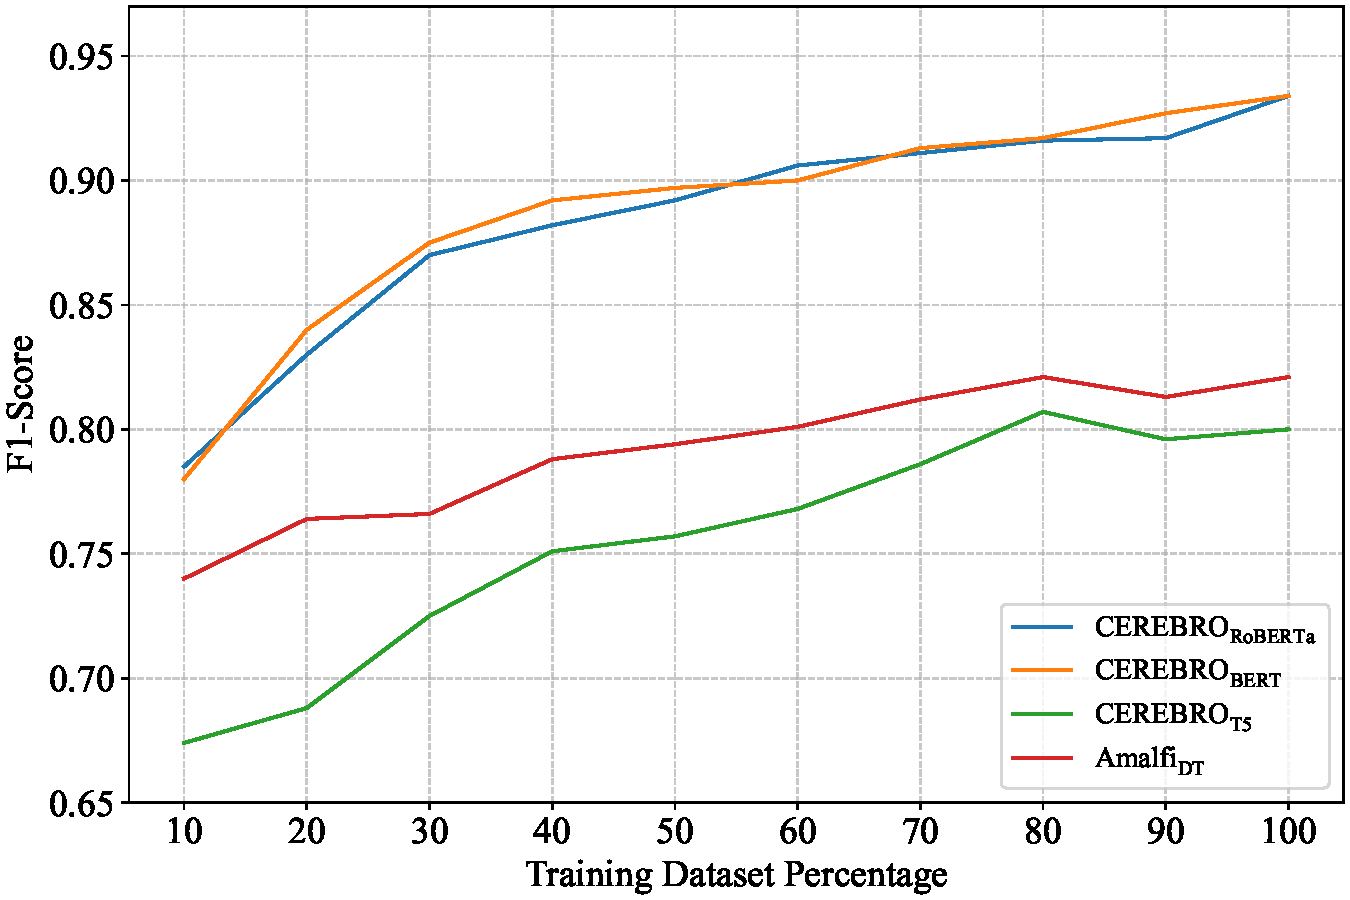
\includegraphics[width=\linewidth]{fig/data_percentage_mix_to_pypi.pdf}
        \vspace*{-5pt}
        \caption{\tosemminorrevision{PyPI Packages as the Testing Dataset}}
        \label{fig:mixed_to_pypi}
    \end{subfigure}
    \hfill % Adds horizontal space between the figures
    \begin{subfigure}[b]{0.49\linewidth}
        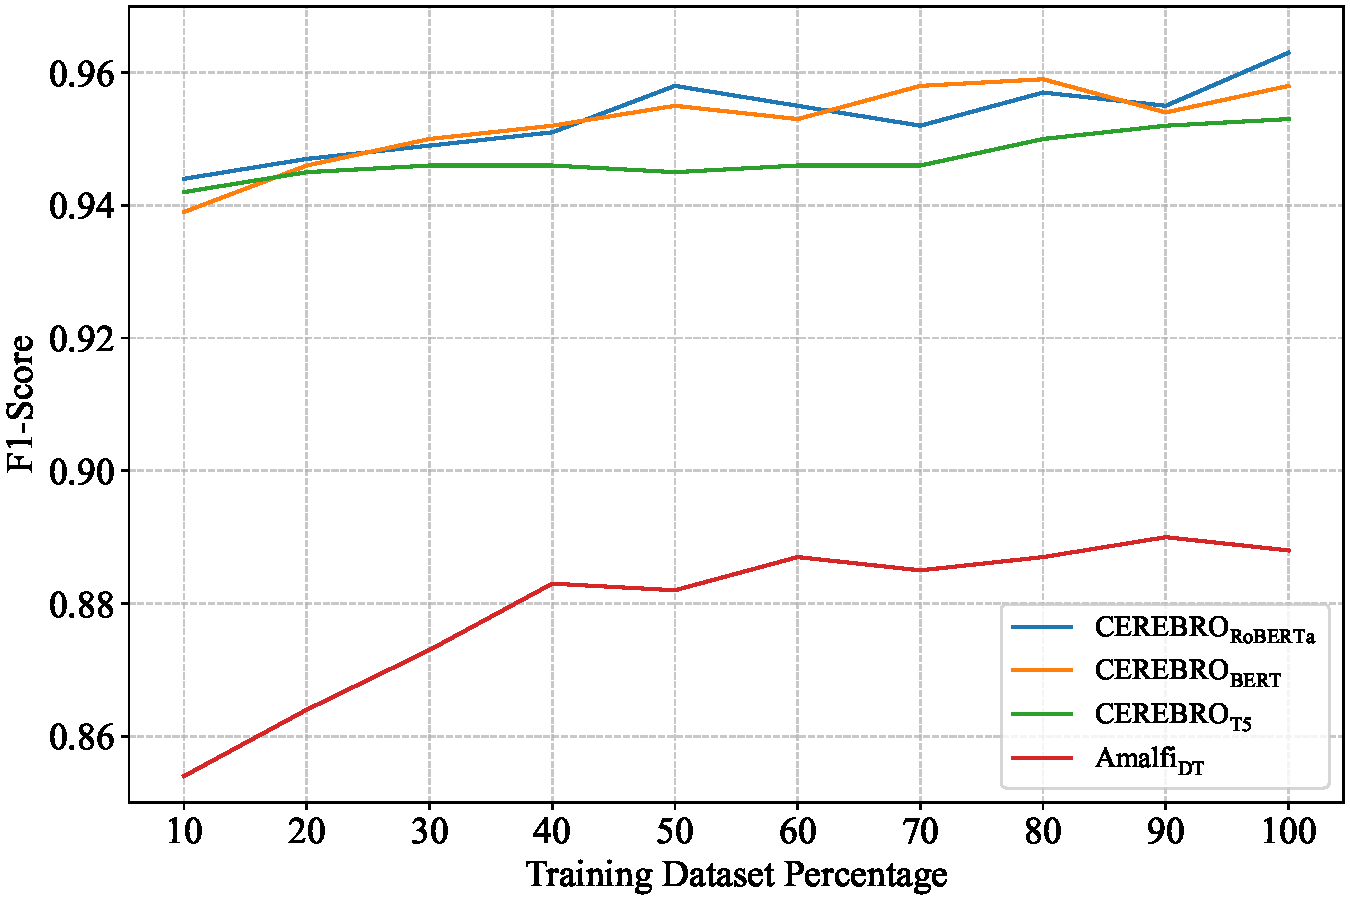
\includegraphics[width=\linewidth]{fig/data_percentage_mix_to_npm.pdf}
        \vspace*{-5pt}
        \caption{\tosemminorrevision{NPM Packages as the Testing Dataset}}
        \label{fig:mixed_to_npm}
    \end{subfigure}
    \vspace{-10pt}
    \caption{\tosemminorrevision{Effectiveness of \tool$_{BERT}$, \tool$_{RoBERTa}$, \tool$_{T5}$ and \textsc{Amalfi}$_{DT}$ in Different Scales of Dataset}}
    \label{fig:dataset_scale}
\end{figure*}

\subsection{\tosemrevision{Dataset Scale Evaluation (RQ3)}}

% \tosemrevision{
% We evaluate the effectiveness of \tool with different dataset scales. Specifically, we sample 10\%, 20\%, 30\%, 40\%, 50\%, 60\%, 70\%, 80\%, 90\% and 100\% of the original dataset to train \tool and \textsc{Amalfi}$_{DT}$ on the bi-lingual scenario. We measure the F1-Score on the same testing dataset in RQ1 with different dataset scales.
% }
% 图a 10%: 0.785 - 0.74 100%: 0.934 - 0.821
% 图b 10%: 0.944 - 0.854 avg:

\tosemrevision{Figure~\ref{fig:dataset_scale} presents the results of our dataset scale evaluation. Overall, \tool$_{BERT}$ and \tool$_{RoBERTa}$ consistently outperform the state-of-the-art by a significant margin in both PyPI and NPM packages, even with limited dataset scales (i.e., 10\%, 20\%). In Figure~\ref{fig:dataset_scale}(a), \tool$_{BERT}$ and \tool$_{RoBERTa}$ exhibit similar F1-Scores as the dataset scale changes. \tool$_{RoBERTa}$ outperforms \textsc{Amalfi}${DT}$ by an F1-Score of 0.045 at the 10\% scale. As the dataset scale increases, \tool$_{RoBERTa}$ further widens the gap, surpassing \textsc{Amalfi}${DT}$ with an F1-Score of 0.113 at the 100\% scale. In Figure~\ref{fig:dataset_scale}(b), \tool$_{BERT}$, \tool$_{RoBERTa}$, and \tool$_{T5}$ exhibit similar F1-Scores as the dataset scale changes. \tool$_{RoBERTa}$ outperforms \textsc{Amalfi}${DT}$ by an F1-Score of 0.09 at the 10\% scale. As the dataset scale increases, \tool$_{RoBERTa}$ further keeps the gap, achieving an average F1-Score difference of 0.072 across remaining dataset scales.} 
\tosemminorrevision{We also observe that as the training dataset increases, the F1-score improvement for NPM packages is relatively smaller compared to PyPI packages. This is primarily due to the differing levels of package diversity between the two ecosystems. As shown in Fig. \ref{fig:malware_category}, a larger proportion of NPM packages focus on information stealing. Consequently, models trained on NPM packages quickly learn and generalize malicious patterns from smaller datasets than those for PyPI, resulting in better performance at lower data percentages and smaller incremental gains as the dataset scale increases.}



% Despite the differences in the source code between packages, the frequent and consistent use of similar APIs related to networking and file system operations introduces shared patterns in the behavior sequence extracted. 
% This consistency allows models to 

% As a result, the models perform well at lower data percentages because they have already captured the key malicious behaviors present across many NPM packages. In contrast, the variation in PyPI package behaviors is higher, leading to a greater improvement in performance as the data scale increases.}

% \tosemminorrevision{It should be noted that for both PyPI and NPM packages, the F1-Score steadily increases as the dataset scale increases. However, the rate of improvement in F1 score between 10\% and 100\% of training data for NPM packages (an average of 0.021) is considerably smaller compared to the improvement seen for PyPI packages (an average of 0.128). This phenomenon can be attributed to the fact that most malicious NPM packages are associated with information stealing. Despite the differences in the source code between packages, the frequent and consistent use of similar APIs related to networking and file system operations introduces shared patterns in the behavior sequence extracted. This consistency allows models to quickly learn and generalize malicious patterns even with smaller datasets. As a result, the models perform well at lower data percentages because they have already captured the key malicious behaviors present across many NPM packages. In contrast, the variation in PyPI package behaviors is higher, leading to a greater improvement in performance as the data scale increases.}

% summary要改吗
\tosemrevision{\textbf{Summary.} The effectiveness of our approach maintains an advantage over state-of-the-art across different dataset scales. \tool$_{RoBERTa}$ achieves an F1-Score of \tosemrevision{0.785} in PyPI and \tosemrevision{0.944} in NPM even when the dataset scale is reduced by 90\%, indicating the robustness of \tool in situations with scarce data availability.}


\subsection{Ablation Study (RQ4)}


% We create an ablated version of \tool by removing the Call Graph Generator and Behavior Sequence Generator of the original version. The unordered features from the Feature Extractor are directly transformed into textual descriptions and fed into the BERT. We retrain using the same dataset. 

We train the three ablated versions of \tool in the bi-lingual scenario. As shown in Table~\ref{table:result-ablation}, the ablated version is less effective than the original version.
\tosemrevision{Specifically, the average precision and recall for \tool$_{BERT}$, \tool$_{RoBERTa}$ and \tool$_{T5}$ decrease 1.6\% and 0.6\%, increase 1.6\% and decrease 3.7\%, decrease 1.4\% and 1.9\% for \tool w/o Seq in mono-lingual, cross-lingual and bi-lingual scenarios, respectively.}
\tosemrevision{Similarly, the average precision and recall decrease 1.4\% and 1.2\%, decrease 2.0\% and 33.0\%, decrease 0.5\% and 0.7\% for \tool w/o Text in mono-lingual, cross-lingual and bi-lingual scenarios, respectively.}
\tosemrevision{Further, the average precision and recall decrease 3.0\% and 0.2\%, 27.1\% and 61.4\%, 4.7\% and 3.2\% for \tool w/ DT in mono-lingual, cross-lingual and bi-lingual scenarios, respectively.}
% Similarly, the precision and recall decrease \todo{3.5\%} and \todo{9.1\%} for \tool w/o Text in PyPI, meanwhile \todo{0.9\%} and \todo{2.7\%} in NPM. Notably, the recall gains with a margin rate of \todo{1.4\%} for \tool w/ DT in PyPI. However, this increment is accompanied by a considerable \todo{9.6\%} drop in precision. Further, the precision and recall also decrease \todo{3.1\%} and \todo{0.6\%} for \tool w/ DT in NPM.


\begin{table}[!t]
    \centering
    \tiny
    \caption{\tosemrevision{Evaluation Result on Ablated Versions of \tool (The bold numbers indicate the decreases or increases compared to the non-ablated versions)}}\label{table:result-ablation}
    \vspace{-10pt}
    \begin{tabular}{m{0.30cm}m{0.30cm}m{0.55cm}m{0.55cm}m{0.55cm}m{0.55cm}m{0.55cm}m{0.55cm}m{0.55cm}m{0.55cm}m{0.55cm}m{0.55cm}m{0.55cm}m{0.55cm}m{0.55cm}m{0.55cm}}   
        \noalign{\hrule height 1pt}
        % \multirow{2}{*}{Train}  & \multirow{2}{*}{Test}  & \multicolumn{2}{c}{\tool} & \multicolumn{2}{c}{\textsc{Amalfi-DT}} & \multicolumn{2}{c}{Amalfi-NB} & \multicolumn{2}{c}{Amalfi-SVM}\\
        \multirow{3}{*}{Train} & \multirow{3}{*}{Test} & \multicolumn{6}{c}{\shortstack[l]{\textsc{\tool} w/o Seq}} & \multicolumn{6}{c}{\shortstack[l]{\textsc{\tool} w/o Text}} & \multicolumn{2}{c}{\shortstack[l]{\tool w/ DT}}\\
    \cmidrule(lr){3-8}
    \cmidrule(lr){9-14}
    \cmidrule(lr){15-16}
    & & \multicolumn{2}{c}{\textsc{BERT}} & \multicolumn{2}{c}{\tosemrevision{\textsc{RoBERTa}}} & \multicolumn{2}{c}{\tosemrevision{\textsc{T5}}} &  \multicolumn{2}{c}{\textsc{BERT}} & \multicolumn{2}{c}{\tosemrevision{\textsc{RoBERTa}}} & \multicolumn{2}{c}{\tosemrevision{\textsc{T5}}} & \multirow{2}{*}{Pre.} & \multirow{2}{*}{Rec.} \\
    \cmidrule(lr){3-4}
    \cmidrule(lr){5-6}
    \cmidrule(lr){7-8}
    \cmidrule(lr){9-10}
    \cmidrule(lr){11-12}
    \cmidrule(lr){13-14}
    & & Pre. & Rec. & Pre. & Rec. & Pre. & Rec. & Pre. & Rec. & Pre. & Rec. & Pre. & Rec. & & \\ \hline
    \tosemrevision{PyPI} & \tosemrevision{PyPI} & 91.3\% \textbf{\newline $\downarrow$ 4.5\%} & 87.1\% \textbf{\newline $\downarrow$ 2.3\%} & \tosemrevision{92.1\% \textbf{\newline $\downarrow$ 3.9\%}} & \tosemrevision{86.2\% \textbf{\newline $\downarrow$ 5.5\%}} & \tosemrevision{92.1\% \textbf{\newline $\downarrow$ 1.3\%}} & \tosemrevision{76.1\% \textbf{\newline $\uparrow$ 5.2\%}} & 92.6\% \textbf{\newline $\downarrow$ 3.2\%} & 85.0\% \textbf{\newline $\downarrow$ 4.4\%} & \tosemrevision{90.6\% \textbf{\newline $\downarrow$ 5.4\%}} & \tosemrevision{89.6\% \textbf{\newline $\downarrow$ 2.1\%}} & \tosemrevision{94.1\% \textbf{\newline $\uparrow$ 0.7\%}} & \tosemrevision{76.8\% \textbf{\newline $\uparrow$ 5.9\%}} & \tosemrevision{91.4\% \textbf{\newline $\downarrow$ 4.4\%}} & \tosemrevision{89.4\% \textbf{\newline $\downarrow$ 0.0\%}} \\
    \tosemrevision{NPM} & \tosemrevision{NPM} & 98.0\% \textbf{\newline $\downarrow$ 0.2\%} & 92.2\% \textbf{\newline $\uparrow$ 0.4\%} &\tosemrevision{98.9\% \textbf{\newline $\uparrow$ 0.4\%}} & \tosemrevision{92.1\% \textbf{\newline $\downarrow$ 0.8\%}} & \tosemrevision{98.8\% \textbf{\newline $\downarrow$ 0.1\%}} & \tosemrevision{90.4\% \textbf{\newline $\downarrow$ 0.6\%}} & 98.1\% \textbf{\newline $\downarrow$ 0.1\%} & 90.4\% \textbf{\newline $\downarrow$ 1.4\%} & \tosemrevision{97.7\% \textbf{\newline $\downarrow$ 0.8\%}} & \tosemrevision{90.4\% \textbf{\newline $\downarrow$ 2.5\%}} & \tosemrevision{99.1\% \textbf{\newline $\uparrow$ 0.2\%}} & \tosemrevision{88.3\% \textbf{\newline $\downarrow$ 2.7\%}} &  \tosemrevision{96.6\% \textbf{\newline $\downarrow$ 1.6\%}} & \tosemrevision{92.2\% \textbf{\newline $\uparrow$ 0.4\%}} \\
    \hline % \% \textbf{\newline $\downarrow$ \%}
    \tosemrevision{NPM} & \tosemrevision{PyPI} & 77.3\% \textbf{\newline $\uparrow$ 5.3\%} & 36.0\% \textbf{\newline $\downarrow$ 13.1\%} & \tosemrevision{76.7\% \textbf{\newline $\uparrow$ 1.6\%}} & \tosemrevision{42.1\% \textbf{\newline $\downarrow$ 2.0\%}} & \tosemrevision{64.7\% \textbf{\newline $\downarrow$ 0.5\%}} & \tosemrevision{67.6\% \textbf{\newline $\uparrow$ 4.2\%}} & 93.7\% \textbf{\newline $\uparrow$ 21.7\%} & 18.5\% \textbf{\newline $\downarrow$ 30.6\%} & \tosemrevision{64.2\% \textbf{\newline $\downarrow$ 10.9\%}} & \tosemrevision{2.0\% \textbf{\newline $\downarrow$ 42.1\%}} & \tosemrevision{88.0\% \textbf{\newline $\uparrow$ 22.8\%}} & \tosemrevision{8.4\% \textbf{\newline $\downarrow$ 55.0\%}} & \tosemrevision{49.5\% \textbf{\newline $\downarrow$ 22.5\%}} & \tosemrevision{11.0\% \textbf{\newline $\downarrow$ 38.1\%}} \\
    \tosemrevision{PyPI} & \tosemrevision{NPM}  & 49.2\% \textbf{\newline $\uparrow$ 7.3\%} & 92.2\% \textbf{\newline $\downarrow$ 0.8\%} & \tosemrevision{38.3\% \textbf{\newline $\downarrow$ 8.2\%}} & \tosemrevision{87.2\% \textbf{\newline $\downarrow$ 5.5\%}} & \tosemrevision{41.3\% \textbf{\newline $\uparrow$ 3.8\%}} & \tosemrevision{86.0\% \textbf{\newline $\downarrow$ 4.9\%}} & 41.8\% \textbf{\newline $\downarrow$ 0.1\%} & 94.0\% \textbf{\newline $\uparrow$ 1.0\%} & \tosemrevision{28.0\% \textbf{\newline $\downarrow$ 18.5\%}} & \tosemrevision{98.9\% \textbf{\newline $\uparrow$ 6.2\%}} & \tosemrevision{10.6\% \textbf{\newline $\downarrow$ 26.9\%}} & \tosemrevision{13.6\% \textbf{\newline $\downarrow$ 77.3\%}} &  \tosemrevision{10.2\% \textbf{\newline $\downarrow$ 31.7\%}} & \tosemrevision{8.4\% \textbf{\newline $\downarrow$ 84.6\%}} \\
    \hline
    \multirow{2}{*}{Mixed} & PyPI & 92.3\% \textbf{\newline $\downarrow$ 2.7\%} & 86.2\% \textbf{\newline $\downarrow$ 5.8\%} & \tosemrevision{93.4\% \textbf{\newline $\downarrow$ 2.7\%}} & \tosemrevision{88.3\% \textbf{\newline $\downarrow$ 2.6\%}} & \tosemrevision{92.6\% \textbf{\newline $\downarrow$ 2.0\%}} & \tosemrevision{71.3\% \textbf{\newline $\uparrow$ 1.7\%}} & 95.5\% \textbf{\newline $\uparrow$ 0.5\%} & 86.0\% \textbf{\newline $\downarrow$ 6.0\%} & \tosemrevision{94.7\% \textbf{\newline $\downarrow$ 1.4\%}} & \tosemrevision{87.4\% \textbf{\newline $\downarrow$ 3.5\%}} & \tosemrevision{92.9\% \textbf{\newline $\downarrow$ 1.7\%}} & \tosemrevision{82.0\% \textbf{\newline $\uparrow$ 12.4\%}} &  90.5\% \textbf{\newline $\downarrow$ 4.5\%} & 86.6\% \textbf{\newline $\downarrow$ 5.4\%} \\
     & NPM  & 98.2\% \textbf{\newline $\downarrow$ 0.5\%} & 91.8\% \textbf{\newline $\downarrow$ 1.2\%} & \tosemrevision{98.6\% \textbf{\newline $\downarrow$ 0.3\%}} & \tosemrevision{91.7\% \textbf{\newline $\downarrow$ 2.2\%}} & \tosemrevision{98.9\% \textbf{\newline $\downarrow$ 0.0\%}} & \tosemrevision{90.9\% \textbf{\newline $\downarrow$ 1.1\%}} & 98.7\% \textbf{\newline $\downarrow$ 0.0\%} & 91.1\% \textbf{\newline $\downarrow$ 1.9\%} & \tosemrevision{98.3\% \textbf{\newline $\downarrow$ 0.6\%}} & \tosemrevision{91.1\% \textbf{\newline $\downarrow$ 2.8\%}} & \tosemrevision{98.8\% \textbf{\newline $\downarrow$ 0.1\%}} & \tosemrevision{89.5\% \textbf{\newline $\downarrow$ 2.5\%}} & 93.9\% \textbf{\newline $\downarrow$ 4.8\%} & 92.0\% \textbf{\newline $\downarrow$ 1.0\%} \\
    \noalign{\hrule height 1pt}
    \end{tabular}
\end{table}

\begin{table*}[!t]
    \centering
    \footnotesize
    \caption{\new{Result of Real-World Malicious Package Detection \todel{Over \todo{Six} Weeks}}}\label{table:monitor-stats}
    \vspace{-10pt}
    \begin{tabular}{m{1.1cm}m{1.2cm}m{2.2cm}m{1.2cm}m{1.1cm}m{1.1cm}m{1.5cm}m{1.5cm}}
        \noalign{\hrule height 1pt}
        Package Registry & Time Period & Newly Published Package Versions & Flagged by \tool & False Positives & True Positives & Thank Letters & Removed Before Report \\
        \hline
        \multirow{7}{*}{PyPI}
        & March & 104,512 & 750 & 521 & 229 & 173 & 56 \\
        & April & 101,415 & 661 & 560 & 101 & 0 & 101 \\
        & May & 78,528 & 422 & 324 & 98 & 30 & 68 \\
        & June & 102,088 & 768 & 595 & 173 & 0 & 173 \\
        & July & 101,600 & 720 & 670 & 50 & 10 & 40 \\
        & August & 56,561 & 298 & 283 & 15 & 14 & 1 \\
        & September & 25,193 & 101 & 88 & 13 & 4 & 9 \\
        & October & 29,596 & 16 & 12 & 4 & 1 & 3 \\
        \cline{2-8}
        & Total & 599,493 & 3,746 & 3,053 & 683 & 232 & 451 \\
        \hline
        \multirow{6}{*}{NPM}
        & April & 130,697 & 325 & 178 & 147 & 147 & 0 \\
        & May & 39,094 & 145 & 88 & 57 & 35 & 22 \\
        & June & 28,764 & 256 & 145 & 111 & 0 & 111 \\
        & July & 34,626 & 244 & 155 & 89 & 44 & 45 \\
        & August & 33,013 & 514 & 314 & 200 & 131 & 69 \\
        & September & 27,350 & 374 & 254 & 120 & 91 & 29 \\
        & October & 30,601 & 372 & 297 & 75 & 27 & 48 \\
        \cline{2-8}
        & Total & 324,145 & 2,230 & 1431 & 799 & 475 & 324 \\
        \hline
        \noalign{\hrule height 1pt}
    \end{tabular}
\end{table*}


\textbf{\textit{Summary.}} Generating behavior sequence, transforming behavior sequence into textual description, and feeding textual description into a classifier fine-tuned from a \tosemrevision{pre-trained language model} are all effective in detecting malicious packages. \tosemrevision{Averagely, the ablated versions of \tool decrease 4.5\% in precision and 11.8\% in recall.}


% The results of the ablation study is shown in Table. \ref{table:ablation}. 
% 
% \begin{table}[!t]
%     \centering
%     \footnotesize
%     \caption{Ablation Results}\label{table:ablation}
%     % \vspace{-10pt}
%     \begin{tabular}{m{1cm}m{1cm}m{0.6cm}m{0.6cm}m{0.6cm}m{0.6cm}m{0.6cm}m{0.6cm}m{0.6cm}m{0.6cm}m{0.6cm}}   
%         \noalign{\hrule height 1pt}
%         \multirow{2}{*}{Train} & \multirow{2}{*}{Test}  & \multicolumn{2}{c}{\tool} & \multicolumn{2}{c}{\textsc{$\tool_{A}$}} \\
%     % \cmidrule(lr){3-6}
%     % \cmidrule(lr){7-10}
%     % & & Pre. & Rec. & F1 & Acc. & Pre. & Rec. & F1 & Acc.  \\ 
%     % \noalign{\hrule height 1pt}
%     % Mixed & NPM & 99.1\% & 91.5\% & 95.1\% & 97.3\% & 94.7\% & 91.0\% & 92.8\% & 95.9\%  \\
%     % Mixed & PyPI & 97.0\% & 82.2\% & 88.8\% & 96.4\% & 93.3\% & 70.7\% & 79.8\% & 93.8\%  \\
%     \cmidrule(lr){3-4}
%     \cmidrule(lr){5-6}
%     & & Pre. & Rec. & Pre. & Rec.  \\ 
%     \noalign{\hrule height 1pt}
%     Mixed & PyPI & 97.0\% & 82.2\% & 93.3\% & 70.7\% \\
%     Mixed & NPM & 99.1\% & 91.5\% & 94.7\% & 91.0\% \\
%     \noalign{\hrule height 1pt}
%     \end{tabular}
% \end{table}

\subsection{Real-World Usefulness Evaluation (RQ5)}

To evaluate the practical usefulness of \tool in analyzing newly published package versions in real-world registries,~we design a monitoring system that first monitors and crawls newly published package versions from PyPI and NPM and then runs \tool against the crawled package versions. Our monitoring system has lasted over \new{\todo{8} months for PyPI and \todo{7} months for NPM}\todel{\todo{six} weeks}.

% Then, we evaluate \tool's adaptiveness in acquiring knowledge from new packages by retraining on an updated dataset adding with new packages. Further, we also characterize the detected malicious packages.

\textbf{Overall Usefulness Result.} \new{In total,} \tool scans \new{923,638} newly published package versions, and flags \new{3,746} PyPI package versions and \new{2,230} NPM package versions as potentially malicious, as reported in Table \ref{table:monitor-stats}.~We~first manually validate each flagged package version, and confirm \new{683} PyPI package versions and \new{799} NPM package versions as true positives. Then, following responsible disclosure process, we promptly report these package versions to administrators of the official PyPI and NPM teams. At the time of reporting, \new{451} PyPI package versions and \new{324} NPM package versions have already been removed. The PyPI and NPM teams confirm the remaining \new{232} PyPI package versions and \new{475} NPM package versions as malicious, and remove all of them. Thus, we receive~\new{232} and \new{457} thank letters from PyPI and NPM.

% We manually validate each packages and find that \todo{306} PyPI packages and \todo{198} NPM packages are true positives. We report to PyPI and NPM administrators as soon as the malicious packages have gone through the manual validation process. In total, we receive \todo{203} thank letters from PyPI and \todo{183} thank letters from NPM. The rest packages are removed before we sending the report. 

\textbf{False Positive Analysis.} As shown in Table \ref{table:monitor-stats}, the false positive rate is \new{81.5\%}\todel{\todo{73.9\%}} for PyPI and \new{64.2\%}\todel{\todo{58.3\%}} for NPM, which is actually high. It is worth mentioning that it takes one~of~our authors around one hour to manually analyze and confirm the flagged package versions every day, which is still acceptable. After analyzing all the false positives, we identify~four major types of benign packages that are flagged as malicious,~as~their behavior sequences are similar to malicious ones. 

First, some benign packages encapsulate RESTful APIs, which enable data transmission~to~remote servers. Their behavior sequences consist of features about \textit{Information Reading} and \textit{Data Transmission} (e.g., R1, D1, D2 and D3). Second, some benign packages encapsulate CLI commands into Python/JavaScript methods where their behavior sequences resemble those malicious packages in using features about \textit{Payload Execution}. Third, some benign packages behave similarly to Trojans, but their payloads serve benign purposes. Normally, their behavior sequences resemble Trojans by starting with D1 and D3, then undertaking intermediate actions such as R1 and R4, and ending with P2 and P3. Last, some benign packages consist of a single meta utility module that incorporates features ranging from \textit{Information Reading}, \textit{Data Transmission}, \textit{Encoding} to \textit{Payload Execution}. It causes \tool to recognize parts of behavior~sequences as similar to those of malicious packages.


\new{\textbf{False Negative Analysis.} To measure false negatives of \tool, we reached out to package registries. However, PyPI replied that they did not maintain a malicious package list and NPM refused to share the list. Therefore, we try to use state-of-the-art detectors to identify true positives. Specifically, we employ \textsc{Amalfi}~\cite{sejfia2022practical} to identify potentially malicious packages~during the same monitoring time period. It flagged \todo{41,434} PyPI package versions and \todo{1,930} NPM package versions as potentially malicious. Then, we undertake a manual inspection process with a sampling rate of 95\% confidence level and 5\% error margin, which results in \todo{381} PyPI packages and \todo{164} NPM packages. After manual validation, we identify \todo{9} malicious PyPI packages and \todo{45} malicious NPM packages. Remarkably, only \todo{2} PyPI packages and \todo{5} NPM packages went undetected by \tool. It indicates that the false negative rate of \tool is relatively low in real-world detection.}


% PyPI Mar.03 - Mar. 12
% test: Mar. 13 Mar. 22

% NPM: mar. 25 -Apr. 03
% test: Apr. 04 - Apr. 13


\begin{table}[t]
    \footnotesize
    \centering
    \caption{\new{Result of Incremental Learning}}\label{table:result-after-retrain}
    \vspace{-10pt}
    \begin{tabular}{m{2.6cm}m{2.6cm}m{1.6cm}m{1.0cm}}
        \toprule
        % npm_first_10 & npm_second_10 & pypi_first_10 & pypi_second_10 \\
        % 204 & 121 & 184 & 285 \\
        Added Train (\#) & Time Period  & New Test (\#)  & Pre.\\\hline
        None &  - & \multirow{5}{*}{PyPI (1,135)} & 7.2\% \\
        % & PyPI & 184 & 10 Days &  & 44.0\% \\
        PyPI (750) & March &  & 26.5\% \\
        Mixed (1,736) & March-April &  & 36.5\% \\
        Mixed (2,303) & March-May &  & 39.0\% \\
        Mixed (3,327) & March-June &  & 58.2\% \\
        % & PyPI &\new{754} & 3 Months &  & \new{65.2}\% \\
        % Mixed (1,380) & Last Three Months &  & 67.1\% \\
        \cline{1-4}
        None & -- & \multirow{5}{*}{NPM (1,504)} & 32.2\%  \\
        % & NPM &204 & 10 Days &   & 79.7\% \\
        % Mixed (388) & First Days &  & 85.0\% \\
        % & NPM &\new{626} & 3 Months &  & \new{90.3}\% \\
        % Mixed (1,380) & Last Three Months &  & 87.8\% \\
        PyPI (750) & March &  & 76.3\% \\
        Mixed (1,736) & March-April &  & 80.3\% \\
        Mixed (2,303) & March-May &  & 80.2\% \\
        Mixed (3,327) & March-June &  & 80.7\% \\
        % PyPI+NPM+PyPI(Mar. 03 - Mar. 12, 184) & PyPI(Mar. 13 - Mar. 22, 285)  & 68.6\% \\
        % PyPI+NPM & NPM(Apr. 04 - Apr. 13, 121)   & 56.4\% \\
        \bottomrule
    \end{tabular}
\end{table}


\textbf{Incremental Learning Result.} As we are continuously confirming and accumulating true positives and false positives of malicious packages based on our monitoring system, one potential way to reduce false positives is to adopt incremental learning on such true positives and false positives. \new{To this~end, we add the true positives and false positives confirmed\tosemrm{during the first ten days and the \tosem{first} three months} during our monitoring \tosem{from March to June} as two incremental datasets for retraining.} \tosem{In particular, we add 750 packages from March, 1,736 packages from March to April, 2,303 packages from March to May and 3,327 packages from March to June, as reported in the third to sixth row, and eight to eleven row under the column of \textit{Added Train} in Table~\ref{table:result-after-retrain}. Note that the added training dataset for March contains only PyPI packages because monitoring NPM packages starts from April.} \new{Then, we retrain four models of \tool by augmenting the original mixed training dataset with the new mixed PyPI and NPM packages.} Finally, we select true positives and false positives confirmed during our monitoring from July to October as the new testing dataset. In particular, there are \todo{1,135} PyPI packages \new{and \todo{1,504} NPM packages } as reported in the third column in Table \ref{table:result-after-retrain}. 

Overall, by incorporating new malicious and benign packages into the training dataset, the precision of \tool~improves significantly. Specifically, when \tool is retrained with new mixed packages, the precision of detecting malicious PyPI packages reaches \new{58.2\%}, while the precision of detecting malicious NPM packages reaches \new{80.7\%}, achieving a precision increase of \new{51.0\%}\todel{\todo{22.7\%}} for PyPI packages and \todel{\todo{28.6\%}}\new{48.5\%} for NPM packages in total.


% \begin{table}[!t]
%     \centering
%     \small
%     \caption{Triggering Scenarios of New Malicious Packages}\label{table:trigger_type}
%     % \vspace{-10pt}
%     \begin{tabular}{m{2.2cm}m{2.7cm}m{2.2cm}}
%         \noalign{\hrule height 1pt}
%         Package Registry & Triggering Scenarios & Package Number \\\hline
%         \multirow{3}{*}{PyPI} 
%         & Install-Time & 177 \\
%         & Import-Time & 103 \\
%         & Run-Time & 26 \\ % 306
%         \hline
%         \multirow{3}{*}{NPM} 
%         & Install-Time & 189 \\
%         & Import-Time & 7 \\ %196
%         & Run-Time & 0 \\
%         \noalign{\hrule height 1pt}
%     \end{tabular}
% \end{table}

% \begin{table}[!t]
%     \centering
%     \footnotesize
%     \caption{\new{Triggering Scenarios of New Malicious Packages}}\label{table:trigger_type}
%     \vspace{-10pt}
%     \begin{tabular}{m{2.95cm}m{2.2cm}m{2.95cm}m{2.2cm}}
%         \noalign{\hrule height 1pt}
%         \multicolumn{2}{c}{PyPI} & \multicolumn{2}{c}{NPM} \\
%         \cmidrule(lr){1-2}
%         \cmidrule(lr){3-4}
%         Triggering Scenarios & Package Number & Triggering Scenarios & Package Number \\
%         \cmidrule(lr){1-2}
%         \cmidrule(lr){3-4}
%         % \hline
%         % \multirow{3}{*}{PyPI} 
%          Install-Time & 477 & Install-Time & 758  \\
%          Import-Time & 161 & Import-Time & 17\\
%          Run-Time & 45 & Run-Time & 24\\ % 306
%         % \hline
%         % \multirow{3}{*}{NPM} 
%         % \\
%         % \\ %196
%         %  \\
%         \noalign{\hrule height 1pt}
%     \end{tabular}
% \end{table}

% \begin{table}[!t]
%     \centering
%     \footnotesize
%     \caption{\new{Malicious Intentions of New Malicious Packages}}\label{table:malware_category}
%     \vspace{-10pt}
%     \begin{tabular}{m{2.9cm}m{2.2cm}|m{2.9cm}m{2.2cm}}
%         \noalign{\hrule height 1pt}
%           Malicious Intentions & Package Number & Malicious Intentions & Package Number  \\\hline
%           Stealing  & 1,051 &  Implanting Appearingly Benign Payload &  22  \\
%         %   Personal information stealer & 65 & 28\\
%           Sabotaging & 105      &Ransomware & 1  \\
%           Proof of Concept & 117  & Unknown & 142 \\
%         %   Privilege escalation & 2& 2\\
%          Backdoor & 44  &    &  \\
%         \noalign{\hrule height 1pt}
%     \end{tabular}
% \end{table}

\begin{figure*}[!t]
    \centering
    \begin{subfigure}[t]{0.45\linewidth} % 将 [htbp] 改为 [t] 使得两幅图顶端对齐
        \centering
        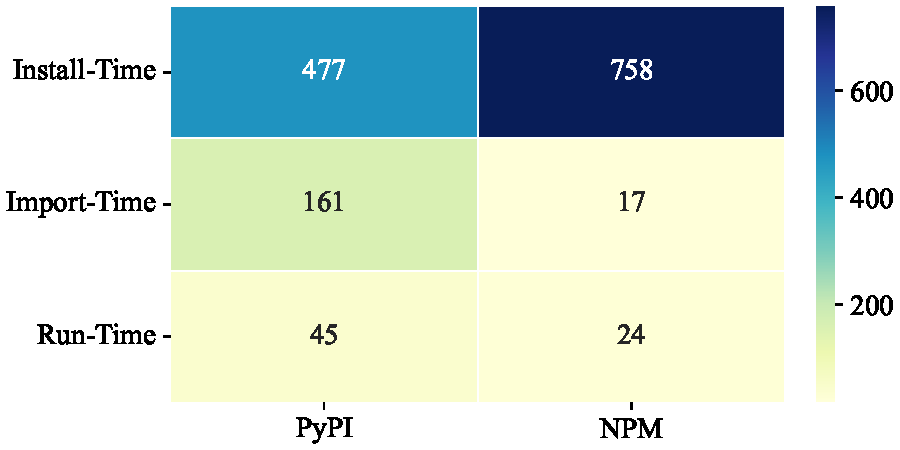
\includegraphics[width=\linewidth]{fig/triggering_scenarios_heatmap.pdf}
        \caption{\tosemminorrevision{Triggering Scenarios of Malicious Packages}}
        \label{fig:trigger_type}
    \end{subfigure}
    \hfill % 增加水平间距
    \begin{subfigure}[t]{0.45\linewidth} % 同样修改为 [t] 确保顶端对齐
        \centering
        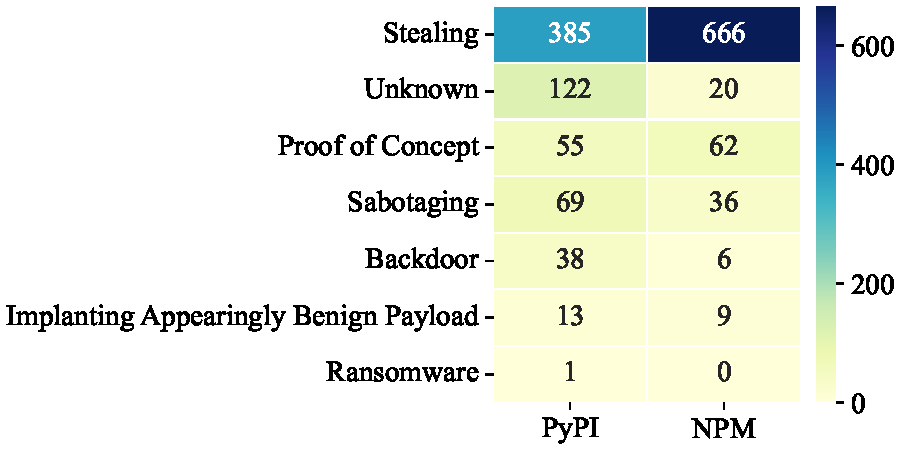
\includegraphics[width=\linewidth]{fig/malicious_intentions_heatmap_npm_pypi.pdf}
        \caption{\tosemminorrevision{Malicious Intentions of Malicious Packages}}
        \label{fig:malware_category}
    \end{subfigure}
    \vspace{-7pt}  % 调整垂直间距，使整个 figure 标题与图片更接近
    \caption{\tosemminorrevision{Triggering Scenarios and Malicious Intentions of New Malicious Packages}} % 总体 caption
    % \label{fig:combined_figure}
\end{figure*}

% \begin{figure*}[!t]
%     \centering
%     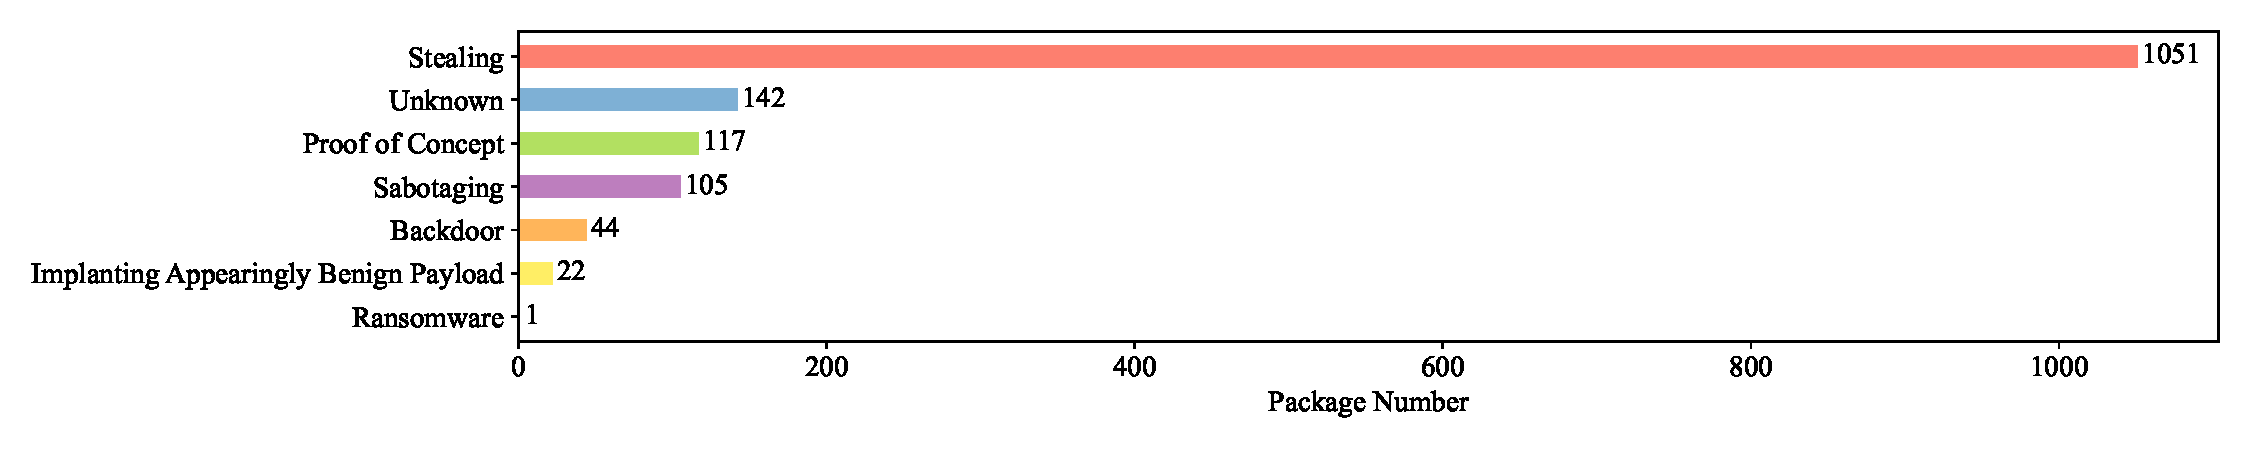
\includegraphics[width=0.95\linewidth]{fig/malicious_intentions.pdf}
%     \vspace{-7pt}
%     \caption{\tosemrevision{Malicious Intentions of New Malicious Packages}}\label{fig:malware_category}
% \end{figure*}

\textbf{Malicious Package Characteristics.} For each of the \new{683} PyPI and \new{799} NPM malicious package versions which are previously unknown, we manually look into their malicious behavior to understand~their~characteristics. On the one hand, we determine their triggering~scenarios, and report the result \tosemrevision{in Figure~\ref{fig:trigger_type}}. We can observe that \new{477 (69.8\%)} of the malicious PyPI package versions and \new{758 (94.9\%)} of the malicious NPM package versions trigger their malicious behavior at install-time. This is reasonable because install-time execution can achieve the highest probability of successfully carrying out attacks. \new{Moreover, a small number of malicious PyPI package versions opt to trigger malicious~behavior other than install-time, accounting~for~\new{161~(23.6\%)} at import-time and 45 (6.6\%) at run-time. Noticeably, there are only \new{17 (2.1\%)} of the malicious NPM package versions that adopt import-time triggering, and \new{24 (\new{3.0\%})} malicious NPM package versions adopt run-time triggering.}

On the other hand, we explore the intentions of malicious package versions by executing them in a sandbox, and present the result in \tosemrevision{Figure~\ref{fig:malware_category}}. Generally, the malicious intentions~include stealing (e.g., personal data or credentials), sabotaging (e.g., shutting down firewalls), proof~of~concept~(which is harmless but to demonstrate something malicious can be done), backdoor (i.e., enabling remote-controlled operations for an attack to exploit an infected machine), implanting appearingly benign payload (e.g., the benign payload might change to be malicious via morphing Trojan), and ransomware. Besides, we fail to execute the payload for \new{142} of the malicious package versions due to non-existent URLs or run-time exceptions, and thus we label their malicious intentions as unknown.

\textbf{\textit{Summary.}} \tool detects \new{683} and \new{799} previously unknown malicious PyPI and NPM package versions. All of them have been removed by the official PyPI and NPM teams, and we also receive \new{707} thank letters from them. Further, by incorporating new malicious and benign packages, \tool learns new knowledge to improve its precision. Besides, most (\new{83.3\%}) of these new malicious package versions execute the malicious behavior at install-time; and most (\new{70.9\%}) of them attempt to steal sensitive information.


% \begin{table}[!t]
%     \centering
%     \caption{Malicious Intentions of the Detected Malicious Packages}\label{table:malware_category}
%     % \vspace{-10pt}
%     \begin{tabular}{m{4.5cm}m{1.5cm}m{1cm}}
%         \noalign{\hrule height 1pt}
%           Malicious Intentions & Package Number & Trojan Number \\\hline
%           Stealing  & 266 & 39\\
%         %   Personal information stealer & 65 & 28\\
%           Proofing of concept & 98  &  0\\
%           Backdoor & 36 & 3 \\
%         %   Privilege escalation & 2& 2\\
%           Implanting appealingly benign payload &  17 & 17 \\
%           Sabotaging & 8 & 8 \\
%           Ransoming & 1 & 0 \\ 
%           Unknown & 76 & 76 \\
%           \hline
%           Total   & 502 & 143 \\
%         \noalign{\hrule height 1pt}
%     \end{tabular}
% \end{table}

% \begin{table}[!t]
%     \centering
%     \small
%     \caption{Malicious Intentions of New Malicious Packages}\label{table:malware_category}
%     % \vspace{-10pt}
%     \begin{tabular}{m{5.2cm}m{2.2cm}}
%         \noalign{\hrule height 1pt}
%           Malicious Intentions & Package Number  \\\hline
%           Stealing  & 266 \\
%         %   Personal information stealer & 65 & 28\\
%           Proof of Concept & 98  \\
%           Backdoor & 36 \\
%         %   Privilege escalation & 2& 2\\
%           Implanting Appearingly Benign Payload &  17 \\
%           Sabotaging & 8 \\
%           Ransomware & 1 \\ 
%           Unknown & 76 \\
%           \hline
%           Total   & 502 \\
%         \noalign{\hrule height 1pt}
%     \end{tabular}
% \end{table}


